\documentclass[fleqn,envcountsame,runningheads,10pt,a4paper]{llncs}
\usepackage[utf8]{inputenc}
\usepackage{enumerate} 
\usepackage{verbatim}
\usepackage{graphicx}
\usepackage{amsmath}
\usepackage{amsfonts}
\usepackage{amssymb}
\usepackage{cite}
\usepackage{pdfpages}
\usepackage{color}
\usepackage{url}
\usepackage{ngerman}
\usepackage{geometry}
\usepackage{hyperref}
\geometry{a4paper,left=30mm,right=30mm,top=35mm,bottom=25mm}

\setlength\parindent{0pt}%Festlegen des Absatzeinzuges
\setlength\mathindent{0pt}%Festlegen des Einzuges für abgesetzte Formeln

\pagestyle{headings}

\begin{document}
%==============================================================================
\title{Per-Circuit TCP-over-IPsec Transport for Anonymous Communication Overlay Networks} 
\titlerunning{Per-Circuit TCP-over-IPsec Transport}
\author{Manuel Schneider\\ms476@pluto.uni-freiburg.de}
\authorrunning{Manuel Schneider}
\institute{Seminar am Lehrstuhl für Kommunikationssysteme \\ Albert-Ludwigs-Universität Freiburg}
\maketitle
%==============================================================================
%\begin{abstract}
%Das Ziel bei der Durchführung des Praxis-Proseminars ist, dass sich die Teilnehmer mit (erweiterten) %Fragestellungen im Bereich Kommunikationssysteme beschäftigen. Der Fokus liegt auf einem %praktischen Zugang zur Thematik.
%\end{abstract}

%==============================================================================
\section{Einleitung}
\label{sec:intro}

Das Internet ist zu einem integralen Bestandteil unserer heutigen Gesellschaft herangewachsen. Es bietet die Möglichkeit, beinahe unabhängig von der Distanz, in Millisekunden Informationen auszutauschen. Viele Dienste die durch das Internet zur Verfügung gestellt werden sind nahezu unentbehrlich geworden. Doch die internationale Vernetzung birgt auch Schattenseiten. Die Kommunikation läuft über eine öffentliche Infrastuktur und die zugrundeliegenden Protokolle wurden nicht mit dem Ziel der Anonymität entworfen.\\

Die Lösung für diese Problematik findet sich in Anonymisierungsdiensten. In diesem Artikel handelt es sich um Anonymisierungsnetzwerke, die als Overlay-Network, implementiert in der Anwendungsschicht, über dem traditionellen Transportprotokoll TCP/IP aufsetzen. Eine Alternative sind Anonymisierungsdienste, die auf VPN basieren. Bei diesen Diensten Verbindet sich der Nutzer per VPN zu einem vertrauenswürdigen Dienstleister und hält somit seine Verbindungsdaten vor den Hosts, zu denen er sich danach verbindet, verborgen. Das Problem bei diesen Diensten ist, dass man vor dem Dienstleister nicht anonym ist. Hingegen ist im Design eines Anonymisierungsnetzwerkes wie zum Beispiel \textsc{Tor} vorgesehen, dass keine Partei die kompletten Verbindungsdaten, bestehend aus Ziel- und Quelladresse kennt.\\

\textsc{Tor} ist das am weitesten verbreitete Netzwerk zur Anonymisierung der Verbingungsdaten. Es wurde 2003 gestartet und seither ständig weiter entwickelt. Das Netzwerk umfasst mittlerweile ca 6500 Knoten und eine kumulierte Bandbreite von ca 6\,GBps\footnote{\url{http://torstatus.blutmagie.de/\#Stats}, Abgerufen am 18.12.2014}.  Die Anonymität im Internet, die durch die Verwendung von \textsc{Tor} gewonnen wird, hat allerdings seinen Preis. Das hohe Verhältnis von Nutzern zu Knotenpunkten im Netzwerk treibt die Netzwerkauslastung an ihre Grenzen. Das ist für den Nutzer spürbar durch eine niedrige Bandbreite und hohe Latenzzeiten. \\

Diese Probleme rühren von einer Schwachstelle im Design, die Joel Reardon und Ian Goldberg in ihrem Artikel ``Improving \textsc{Tor} using a TCP-over-DTLS Tunnel'' addressiert haben. Mit der Idee des TCP-over-DTLS Tunnel stellen die Autoren einen Ansatz vor diese Probleme zu beheben. Die Lösung hat allerdings einen Haken: Die Autoren verwenden eine Userspace TCP Implementierung, deren Lizenz nicht mit der von \textsc{Tor} vereinbar ist. Mit dem Ansatz ``Per-Circuit TCP-over-IPsec Transport'' haben es Joel Reardon und Ian Goldberg geschafft die Performanceprobleme im Tornetzwerk unter Kontrolle zu bekommen, ohne auf die Userspace TCP Implementierung angewiesen zu sein.\\

In dieser Ausarbeitung wird auf das Design und die Evaluierung des ``Per-Circuit TCP-over-IPsec Transport'' eingegangen und zum Schluss dessen Einflüsse auf die Sicherheit des \textsc{Tor} Netzewerkes diskutiert. In Abschnitt \ref{sec:basics} wird auf die Details des Tornetzwerkes eingegangen und ein Einblick in den im TCP-over-DTLS ähnlicher Ansatz zur Lösung des Performanceproblems beschrieben. Zusätzlich werden nötigen Kenntnisse zu IPSec erläutert, die für die Verwendung im PCTCP relevant sind. In Abschnitt \ref{sec:pctcp} wird das von Mashael AlSabah und Ian Goldberg vorgeschlagene Verfahren ``Per-Circuit TCP-over-IPsec Transport'' detailliert beschreiben und evaluiert. In Abschnitt \ref{sec:discussion} werden die Veränderungen im PCTCP, bezüglich der Sicherheit kritisch betrachtet und diskutiert.\\


%==============================================================================
\section{Grundlagen}
\label{sec:basics}

Im Folgenden werden Grundlagen zur Architektur des \textsc{Tor} Netzwerks vermittelt. Der Fokus liegt dabei auf der Kommunikation, speziell dem Verbindungsaufbau im Netzwerk. Diese Details sind notwendig um die Problematik zu verstehen, die für die Performanceeinbußen in \textsc{Tor} verantwortlich sind. Lediglich für PCTCP relevante Themen werden erläutert. Bestandteile von \textsc{Tor} wie zum Beispiel Rendevous-Points und Hidden Services, ein Konzept, das ermöglicht, dass auch der Dienstleister anonym bleiben kann, und Directory Servers, die Knoten die Informationen über die aktiven Knoten im Netzwerk verteilen, werden ausgelassen. Des weiteren wird ein verwandert Ansatz erläutert, der versucht die Performanceprobleme mit UDP zu lösen.

%------------------------------------------------------------------------------
\subsection{TOR}
\label{sec:tor}

%\textsc{Tor} war ürsprunglich ein Akronym für The Onion Router, was bereits Vermutungen über das Konzept verrät, doch darauf wird in Abschnitt \ref{sec:tor} näher eingegangen. 

\textsc{Tor} ist als Overlay Network konzipiert. Das bedeutet, dass die \textsc{Tor} Infrastuktur auf dem weltweit bestehenden TCP/IP Netzwerk aufbaut. Die Knoten im Netzwerk, im Folgenden \textit{Onion Routers}, sind von Freiwilligen betriebene Maschinen auf denen die  \textsc{Tor}-Software läuft, welche als Relay konfiguriert wurde. Zu Beginn melden diese Knoten ihre Existenz bei den \textit{Directory Servern} und warten dann auf Verbindungen von den \textsc{Tor} Clients. Wie schon erwähnt werden die Details der Kommunikation zwischen den Directory Servern und den Onion Routern in dieser Ausarbeitung ausgelassen. Diese Details werden von anderen Teilnehmern in diesem Seminar beschrieben. \textcolor{red}{Welches genau?} Es wird angenommen die Directory Server haben korrekte und vollständige Informationen aller Onion Router. Diese Menge der Onion Router bildet das \textsc{Tor}-Netzwerk.

Die Nutzer des \textsc{Tor}-Netzwerkes nutzen die selbe Software wie die Freiwilligen, die die Relays betreiben, allerdings wird sie als Client konfiguriert benutzt. Im folgenden werden diese Clients \textit{Onion Proxies} genannt. Wenn nun ein Onion Proxy eine anonyme Verbindung ins Internet öffnen möchte, benutzt er das \textsc{Tor}-Netzwerk quasi als Proxy. Die Verbindung wird über das Netzwerk geroutet und der Host zu dem die Verbindung erstellt wird kann nun nur die Verbindungsdaten des Onion Routers sehen, an dem die Verbindung das Netzwerk verlassen hat.\\

\subsubsection{Kommunikation - Cells, Circuits und Streams.}
\label{sec:communication}

Um den Ursprung der Performance Probleme und die Unterschiede zum ``UDP over DTLS'' und ``PCTCP'' zu verstehen müssen die \textsc{Tor} Verbindungen näher im Detail erläutert werden. Das technische Design einer Verbindung in \textsc{Tor} wird nun anhand des Aufbaus eines sogenannten \textit{Cuircuits} gezeigt.

Die Kommunikation im Tornetzwerk wird durch \textsc{Tor} Datenpakete, sogenannte \textit{Cells}, erledigt. Es gibt zwei Arten von Cells. \textit{Control Cells} werden zur direkten Kommunikation mit den Onion Routern verwendet. \textit{Relay Cells} werden für die Übermittlung von Streamdaten und Commandos verwendet. Einige notwendige Cells werden in diesem Abschnitt erläutert, viele sind jedoch für diese Ausarbeitung nicht relevant. Die vollständige Liste der Cells und den genauen Headeraufbau kann in \cite{tor} nachgesehen werden.

Bevor eine Verbindung aufgebaut werden kann muss sich der Onion Proxy zu allererst die Informationen über das Netzwerk bei einem Directory Server holen. Wieder werden die Details zu diesem Vorgang ausgelassen und es wird angenommen, dass der Onion Proxy korrekte und vollständige Informationen über das \textsc{Tor}-Netzwerk hat. Der Onion Proxy sucht sich nun drei Onion Router aus dem Netzwerk aus, über die er die Verbindung routen möchte. Circuits werden inkrementell erstellt. Das heißt, dass bei der Erstellung des Circuits ein Onion Router nach dem anderen dem Circuit hinzugefügt wird.

Um sich nun mit dem ersten Knoten zu verbinden sendet der Onion Proxy ($\textit{OP}$) eine Control Cell an den ersten Onion Router ($\textit{OR}_1$). Diese Control Cell enthält das Commando \textsc{Create}. $\textit{OR}_1$ bestätigt mit einer \textsc{Created} Control Cell. Im Anhang der beiden Cells befinden sich Informationen zum Diffie-Hellman Schlüsselaustausch\cite{dh}. Auf dieses Verfahren wird hier nicht weiter eingegangen, es wird aber angenommen, dass die beiden Kommunikationspartner nun einen symmetrischen Schlüssel $K_{OP,OR_1}$ zur weiteren TLS-verschlüsselten\cite{rfc:tls} Kommunikation ausgehandelt haben. $\textit{OP}$ und OR1 können nun mit $K_{OP,OR_1}$ verschlüsselte Relay Cells austauschen. 

Um den Circuit um einen Onion Router $\textit{OR}_2$ zu erweitern,  sendet $\textit{OP}$ eine \textsc{Extend} Relay Cell an $\textit{OR}_1$. Die \textsc{Extend} Relay Cell enthält Informationen wie die Adresse des neuen Onion Routers $\textit{OR}_2$ und die erste Hälfte eines Diffie-Hellman Handshakes. $\textit{OR}_1$ erstellt eine TCP Verbindung zu $\textit{OR}_2$. Wenn schon eine Verbindung besteht, weil schon ein Circuit existiert, der über die beiden Onion Router läuft, wird diese verwendet. $\textit{OR}_1$ packt die Hälfte des Diffie-Hellman Handshakes von $\textit{OR}_1$ in eine \textsc{Create} Control Cell und sendet diese an $\textit{OR}_2$. Wie im ersten Schritt bekommt $\textit{OR}_1$ eine \textsc{Created} Control Cell von $\textit{OR}_2$ zurück. $\textit{OR}_1$ verpackt die Antwort in eine \textsc{Extended} Relay Cell und leitet sie weiter an $\textit{OP}$. Wichtig ist, dass der Schlüsselaustausch hier zwischen  $\textit{OP}$ und $\textit{OR}_2$ stattgefunden, $\textit{OR}_1$ hat die Daten lediglich weitergeleitet. Der Circuit ist nun um $\textit{OR}_2$ erweitert und $\textit{OP}$ und $\textit{OR}_2$ können nun mit $K_{OP,OR_2}$ wiederum verschlüsselte Relay Cells austauschen. 

Auf diese Weise können beliebig viele weitere Onion Router zu dem Circuit hinzugefügt werden. Üblicherweise werden in der Praxis aber drei Onion Router für einen Circuit verwendet. Tor sieht auch vor dass jede Minute ein neuer Circuit verwendet wird, um neue TCP-Streams durch das Netzwerk zu routen. Da das Erstellen der Circuits lange dauern kann, werden Circuits auf Vorrat erstellt. Alte Circuits werden geschlossen wenn keine aktiven TCP Verbindungen mehr darüber geleitet werden.

Wenn der Circuitaufbau abgeschlossen ist, kann er von den Anwendungen verwendet werden. Wie eingangs erwähnt ist das Netzwerk ein Proxy für den Nutzer. In der Tat agiert auch der Onion Proxy, also die Tor Software auf dem PC, wie ein Proxy. Um Tor zu verwenden muss die Verwendung eines SOCKS Proxy\cite{rfc:socks} eingerichtet werden. Um eine Verbindung zu öffnen leitet die Anwendung die Daten über den SOCKS Proxy an den Onion Proxy weiter, welcher sie wiederum über das TOR Netzwerk bis zum letzten Onion Router weiterleitet. Dieser letzte Onion Router wird auch \textit{Exit Node} genannt. Er erstellt die gewünschte Verbindung und leitet die Antwort an den Onion Proxy beziehungsweise die Anwendungen zurück.

\subsubsection{Cross Circuit Interference Problem.}
\label{sec:crosscircuitinterference} 

Unter den vielen Problemen die Tor bis heute noch hat, ist das Cross Circuit Interference Problem eines der konzeptuell schwerwiegensten.\cite{tor_improvements} Tor leidet unter gewissen Umständen unter hohen Netzwerklatenzen. Für alle Circuits, die über die Verbindung zwischen zwei Onion Router laufen, wird in Tor genau eine TCP Verbindung verwendet. Das führt dazu, dass alle Circuits dem selben TCP-Mechanismus zugrundeliegen. Joel Reardon fand heraus, dass die Latenzen weder beim Empfangen noch vom Verarbeiten der Daten, sondern beim Versenden der Daten in den Output Buffern der TCP Implementiereung entstehen und dass die Ursache für die Latenzen die TCP Congestion Control ist, welche Circuits mit niedriger Bandbreite im Vergleich zu Circuits mit hohem Durchsatz benachteiligt.\cite{tcp-over-dtls-thesis,tcp-over-dtls}






\begin{figure}[htpc]
\centering{
  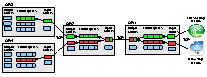
\includegraphics[scale=4]{pics/BufferPic.pdf}
  \caption{Quelle:\cite{pctcp} }
}
\end{figure} 

%------------------------------------------------------------------------------
\subsection{TCP over DTLS}
\label{sec:DTLSrealtedwork}

Einleitung in TCP-over-DTLS, der Ansatz den die Autoren versuchen zu verbessern. \\
Aufzeigen der Probleme und der Punkte an denen die Verbesserungen ansetzen.\\

%------------------------------------------------------------------------------
\subsection{IPSEC}
\label{sec:ipsec}

Basics zu IPSec\\
Erklärungen zu den Subprotokollen:\\
- Authentication Header (AH)\\
- Encapsulating Security Payload (ESP)\\
Erklärungen zu Operationmodes:\\
- transport mode\\
- tunnel mode\\

%==============================================================================
\section{PCTCP}
\label{sec:pctcp}



%------------------------------------------------------------------------------
\subsection{Kernel-mode per-circuit TCP}
\label{sec:kernelmode}

Konzept der Verbindung innerhalb des netzwerks\\
Illustrationen\\
Vorteile des Deployments (Funktion des heterogenen Netzwerks (Plain \textsc{Tor} + PCTCP)\\
änderung am Verbinungsaufbau\\
Resultierende Probleme\\

%------------------------------------------------------------------------------
\subsection{IPSec in PCTCP}
\label{sec:ipsecinpctcp}

- Läsung der Probleme mit IPSec\\ 
- Alternative Läsungen

%------------------------------------------------------------------------------
\subsection{Evaluation}
\label{sec:evaluation}


%==============================================================================
\section{Diskussion}
\label{sec:discussion}



Abgesehen vom Hauptziel seine Nutzer zu anonymisieren, unterliegt das Design von \textsc{Tor} weiteren Zielen. \textsc{Tor} sieht vor in der realen Welt auf eine einfache Weise eingesetzt werden zu können. Mögliche Hürden, zum Beispiel Kernelpatches oder vermeidbare manuelle Interkation, werden umgangen, so dass für den Benutzer die best mögliche Benutzerfreundlichkeit erreicht wird. Grund dafür ist die Tatsache, dass im Kontext von \textsc{Tor} die Benutzerfreundlichkeit in Korrelation zur Sicherheit steht. Die Benutzerfreundlichkeit beeinflusst direkt die Menge der Nutzer des Systems. In \textsc{Tor} werden die Benutzer hinter der Identität anderer Benutzer versteckt. Je weniger Nutzer also im Netzwerk teilmehmen, desto weniger Anonymität kann dem einzelnen Nutzer geboten werden. \textbf{Hier weiter PCTCP ist blöd, weil nicht nutzerfreundlich}\\


Die Verwendung von \textsc{Tor} bietet keine allumfassende Anonymität. Der Nutzer muss auf einen bewussten Umgang mit \textsc{Tor} achten. Es ist wichtig genau zu wissen was \textsc{Tor} bietet und was nicht. So kann sich der Nutzer immernoch selbst durch sein Verhalten im Internet deanonymisieren. \textsc{Tor} bietet auch keine so genannte Protokoll Normalisierung. \textsc{Tor} arbeitet lediglich auf der Netzwerkschicht. Komplexe Protokolle aus höheren Schichten, wie zum Beispiel HTTP, können auch trotz der Verwendung von \textsc{Tor} Informationen über die Identität übertragen. Für diesen Dienst muss auf andere Mittel, wie zum Beispiel den Prokollfilter Privoxy, zurückgegriffen werden. Die Entwickler von \textsc{Tor} setzen ein Bedrohungsmodell fest, in dem angenommen wird, dass ein Feind Teile des Datenverkehrs im Netzwerk überwachen und Datenverkehr erstellen, modifizieren, verwerfen oder verzögern kann. Des weitern kann er Knotenpunkte kompromittieren oder selbst betreiben. In seinem bisherigen Design bietet \textsc{Tor} keine Sicherheit gegen Ende-zu-Ende Attacken\cite{tor}. Unter diesen Annahmen gilt die Anonymität als aufgedeckt, wenn der Feind es geschafft hat ... \textbf{Hier weiter blubbern, weil der sniper angriff genutzt werden kann um neue circuits zu planen. damit kann solang rerouting forciert werden biss alle connecctions übe rkomprommitierte onions laufen}\\


Tor combines all the circuits going between two Tor relays into a single TCP connection. This approach is a
smart idea in terms of anonymity, since putting all circuits on the same connection prevents an observer from
learning which packets correspond to which circuit. But over the past year, research has shown that it’s a
bad idea in terms of performance, since TCP’s backoff mechanism only has one option when that connection
is sending too many bytes: slow it down, and thus slow down all the circuits going across it.
We could fix this problem by switching to a design with one circuit per TCP connection. But that means
that a relay with 1000 connections and 1000 circuits per connection would need a million sockets open. That
number is a problem for even the well-designed operating systems and routers out there.\cite{tor_improvements}



%==============================================================================
\nocite{rfc:socks}
\nocite{rfc:ipsec}
\nocite{rfc:tls}
\nocite{tor}
\nocite{pctcp}
\nocite{tcp-over-dtls}
\nocite{imux}
\nocite{tor_improvements}
\bibliographystyle{splncs}
\bibliography{literatur}
%==============================================================================
\end{document}
